% ==========================================
% Poster: Impact of Adversarial Attacks on SNNs
% Template: Gemini Theme (IITGN 4-Column Layout)
% ==========================================

\documentclass[final]{beamer}

% --- Poster Dimensions ---
\usepackage[size=a1,orientation=landscape,scale=1.0]{beamerposter}
\usetheme{gemini}
\usecolortheme{gemini}
\usepackage{graphicx}
\usepackage{booktabs}
\usepackage{tikz}
\usetikzlibrary{positioning}
\usepackage{pgfplots}
\pgfplotsset{compat=1.14}
\usepackage[most]{tcolorbox}
\usepackage{tabularx}
\usepackage[table]{xcolor}
\usepackage{colortbl}
\setbeamerfont{title}{size=\fontsize{44}{52}\selectfont,series=\bfseries}
% --- Define IITGN colors ---
\providecolor{iitgnblue}{HTML}{003366}
\definecolor{lightiitblue}{HTML}{F2F7FD}
\definecolor{midiitblue}{HTML}{E3EEF9}
\definecolor{deepiitblue}{HTML}{D6E6F6}

% --- Custom tcolorboxes ---
\newtcolorbox{highlightbox}{
  colback=lightiitblue,
  colframe=iitgnblue,
  arc=5pt,
  boxrule=2pt,
  left=15pt, right=15pt, top=10pt, bottom=10pt,
  fontupper=\bfseries,
  center
}
\newtcolorbox{futurebox}{
  colback=lightiitblue,
  colframe=iitgnblue,
  arc=10pt,
  boxrule=2pt,
  left=15pt, right=15pt, top=10pt, bottom=10pt
}

% --- Column Widths ---
\newlength{\colone}
\newlength{\coltwo}
\newlength{\colthree}
\newlength{\colfour}

\setlength{\colone}{0.22\textwidth}
\setlength{\coltwo}{0.23\textwidth}
\setlength{\colthree}{0.30\textwidth}
\setlength{\colfour}{0.21\textwidth}

% --- Header ---
\title{Impact of Adversarial Attacks on Spiking Neural Networks}

\author{\large Pappala Sai Keerthana \and Ravi Bhavana \and Prof.\ Manisha Padala}

\institute{\large Indian Institute of Technology Gandhinagar}

% --- Logos ---
\logoleft{%
  \makebox[0pt][l]{%
    \hspace*{2cm}%
    \IfFileExists{image.png}{%
      
\includegraphics[height=7cm]{image.png}%
    }{%
      \hspace{7cm}%
    }%
  }%
}

\logoright{%
  \makebox[0pt][r]{%
    \hspace*{5cm}%
    \IfFileExists{logo1.png}{%
      
\includegraphics[height=7cm]{logo1.png}%
    }{%
      \hspace{7cm}%
    }%
  }%
}

\begin{document}

\begin{frame}[t]
\begin{columns}[t]

% ============================================================
% COLUMN 1: Introduction & Background
% ============================================================
\begin{column}{\colone}

  \begin{block}{INTRODUCTION}
    \textbf{Overview:} Does spike encoding strategy affect adversarial robustness in SNNs,
    and do SNNs resist attacks differently from ANNs and CNNs?

    

    \begin{highlightbox}
      \centering
      {\textcolor{iitgnblue}{\large \textbf{WHY THIS MATTERS}}}

      
      \begin{itemize}
        \item {\color{gray!120} SNNs are increasingly deployed on edge \& neuromorphic hardware for safety-critical tasks}
        \item {\color{gray!120} Adversarial robustness of SNNs remains understudied vs.\ classical deep nets}
        \item {\color{gray!120} Encoding strategy (rate vs.\ temporal) may introduce implicit robustness but no systematic study exists}
      \end{itemize}
    \end{highlightbox}
  \end{block}

  \begin{block}{SPIKE ENCODING STRATEGIES}
    \begin{minipage}[t]{0.48\linewidth}
      \begin{futurebox}
        {\centering\color{iitgnblue}\bfseries\normalsize Rate Coding\par}
        \vspace{0.4em}\small
        Pixel $x\!\in\![0,1]$ sets spike \textbf{probability} per step:\\[3pt]
        $\;s_t \sim \mathrm{Bernoulli}(x),\; t=1,\ldots,T$\\[4pt]
        Bright $\to$ many spikes. Dense representation.\\
        $T=25$ timesteps (MNIST);\\ $T=10$ (CIFAR rate).
      \end{futurebox}
    \end{minipage}
    \hfill
    \begin{minipage}[t]{0.48\linewidth}
      \begin{futurebox}
        {\centering\color{iitgnblue}\bfseries\normalsize Temporal Coding\par}
        \vspace{0.4em}\small
        Pixel sets \textbf{first-spike latency}:\\[3pt]
        $\;t_{\text{spike}}=\lfloor(1-x)(T-1)\rfloor$\\[4pt]
        Bright $\to$ fires early. \textbf{One spike per neuron.}
        Extremely sparse. $T=25$ (MNIST \& CIFAR \\temporal).
      \end{futurebox}
    \end{minipage}

    
    \begin{figure}
      \centering
      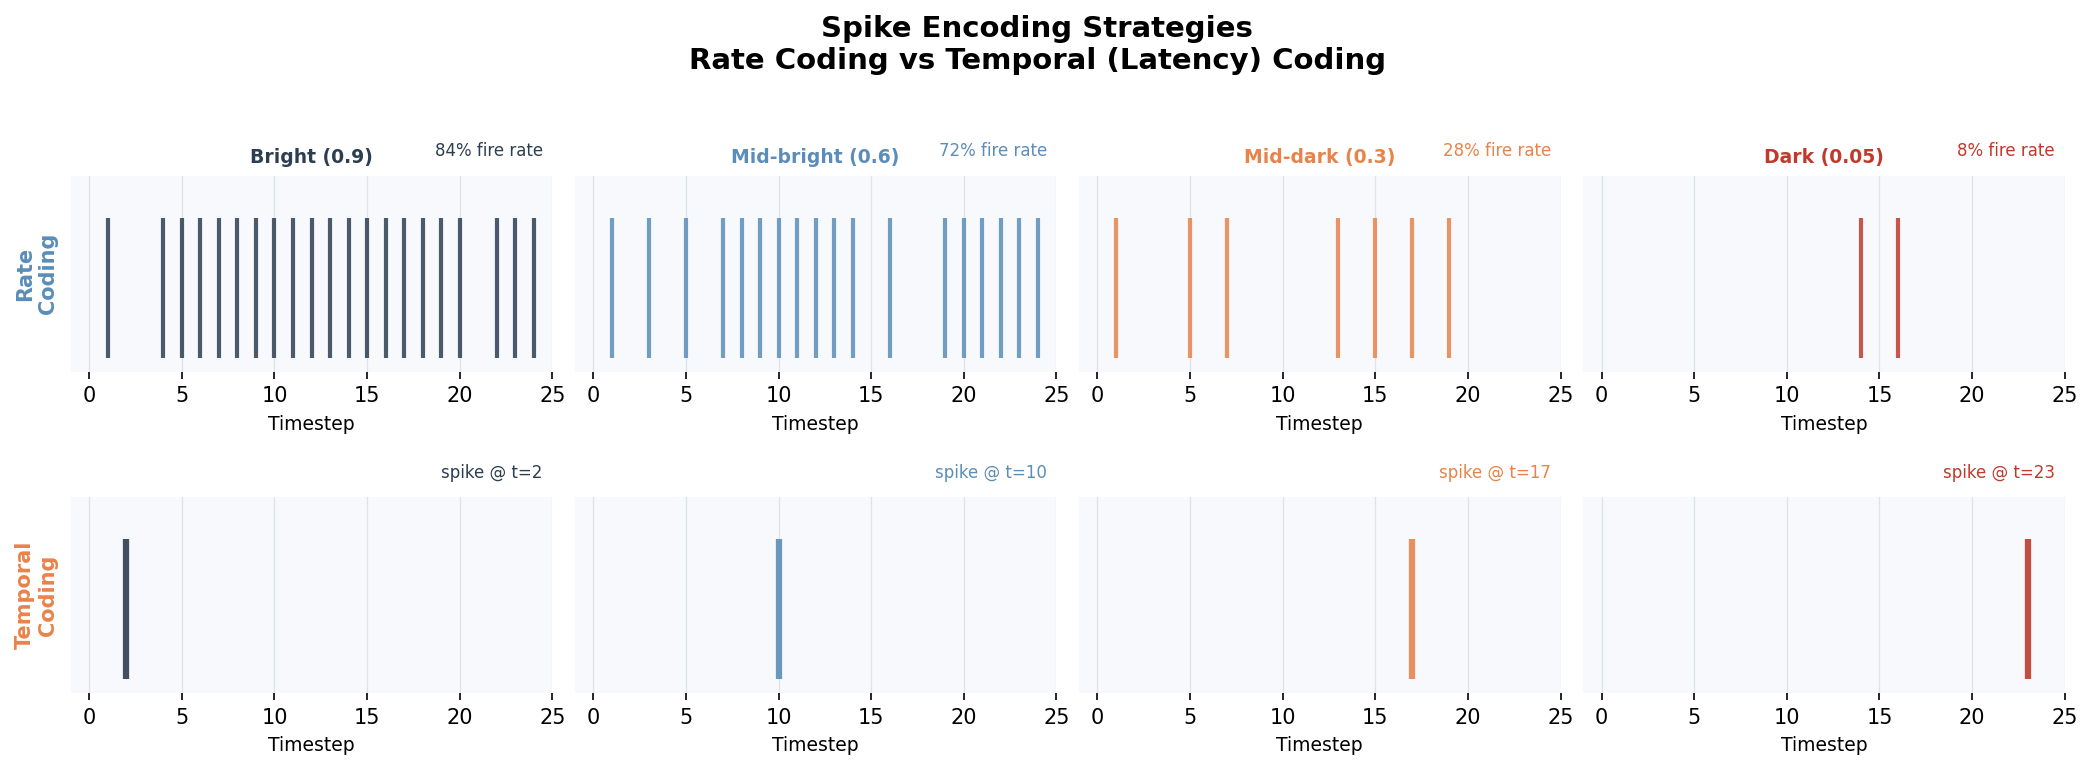
\includegraphics[width=1\linewidth]{fig01_encoding_comparison.png}
    \end{figure}
    \small\textit{*Rate coding uses Bernoulli sampling (MNIST) or deterministic
repeat (CIFAR, pixels   \\ normalized to $\mathbb{R}$).}
  \end{block}

  % FIX 1: Architecture block — corrected channel sizes (64/128/256), dropout (0.4), and LR (2e-3)
  \begin{block}{ARCHITECTURE}
    \begin{futurebox}
      {\centering \usebeamercolor[fg]{block title} \normalsize \bfseries SNN-MNIST (LIF-MLP) \par}
      
      \small
      {\color{iitgnblue!60!black}
        Input (784) $\rightarrow$ FC(1000) $\rightarrow$ LIF $\rightarrow$ FC(10) $\rightarrow$ LIF \\[0.3em]
        % FIX: LR was listed as 10^{-3} but notebook uses lr=2e-3
        $T = 25$ steps $\,\cdot\,$ $\beta = 0.90$ $\,\cdot\,$ Adam ($2\times10^{-3}$) $\,\cdot\,$ Cosine LR 
      }

      

      {\centering \usebeamercolor[fg]{block title} \normalsize \bfseries SPIKING CIFAR (CONV-SNN) \par}
      \vspace{0.4em}
      \small
      {\color{iitgnblue!60!black}
        % FIX: original poster said Conv(32)->Conv(64)->Conv(128); notebook uses 64->128->256
        Conv(64)$\rightarrow$BN$\rightarrow$LIF$\rightarrow$AvgPool \\[0.3em]
        Conv(128)$\rightarrow$BN$\rightarrow$LIF$\rightarrow$AvgPool \\[0.3em]
        Conv(256)$\rightarrow$BN$\rightarrow$LIF$\rightarrow$AvgPool \\[0.3em]
        % FIX: dropout was 0.3 in poster but 0.4 in notebook
        Dropout(0.4) $\cdot$ FC(512)$\rightarrow$BN$\rightarrow$LIF $\cdot$ FC(10)$\rightarrow$LIF \\[0.3em]
        $T_{\text{rate}} = 10,\; \beta=0.50$ $\;\cdot\;$
        $T_{\text{temp}} = 25,\; \beta = 0.90 \\\;\cdot\; \text{Cosine LR (rate } = 1e^{-3},\ \text{temporal} = 5e^{-4})$
        
      }
    \end{futurebox}
  \end{block}

  \begin{block}{SURROGATE GRADIENT}
    Heaviside spike function $\rightarrow$ non-differentiable.
    We replace its derivative with a fast-sigmoid surrogate $\sigma'(U)$
    during backprop :

    \[
      \sigma'(U) = \frac{\text{slope}}{(1 + |\text{slope} \cdot U|)^2}
    \]

    \small\textit{slope = 25 for all models. Temporal attacks use the
    straight-through estimator (STE): continuous pixel image repeated $T$ times
    replaces discrete latency encoding during gradient computation.}
  \end{block}

\end{column}

% ============================================================
% COLUMN 2: Attacks & Results Tables
% ============================================================
\begin{column}{\coltwo}

  \begin{block}{THE SPIKING NEURON MODEL}
    \small
    We use the \textbf{Leaky Integrate-and-Fire (LIF)} model (discrete time):
    % FIX: original poster wrote Ui(t) = βUi(t−1) + ΣWijSj(t) − VthSi(t−1)
    % The reset term should subtract V_th * S_i(t), not S_i(t-1)
    % Also the current convention in snnTorch is:
    %   U[t] = β·U[t-1] + I[t] - S[t-1]   (reset-by-subtraction)
    % We keep the standard poster form but clarify it matches snnTorch
    \[
      U_i[t] = \beta\, U_i[t-1] + \sum_j W_{ij}\, S_j[t] - V_{\text{th}}\, S_i[t-1]
    \]
    \textbf{Integrates input spikes $S_j[t]$, fires when $U_i[t] > V_{th}$,
    resets by subtraction, and decays via leakage factor $\beta$.}
    
  \end{block}

  \begin{block}{MODELS EVALUATED}
    \centering
    \vspace{0.5ex}
    \renewcommand{\arraystretch}{1.6}
    \setlength{\tabcolsep}{10pt}
    \begin{tabularx}{\columnwidth}{>{\raggedright\arraybackslash}X
                                   >{\centering\arraybackslash}X
                                   >{\raggedleft\arraybackslash}X}
      \rowcolor{iitgnblue}
      \textbf{\textcolor{white}{Model Architecture}} &
      \textbf{\textcolor{white}{Dataset}} &
      \textbf{\textcolor{white}{Coding}} \\
      SNN-Rate       & MNIST / CIFAR-10 & Rate (LIF) \\
      \rowcolor{deepiitblue}
      SNN-Temporal   & MNIST / CIFAR-10 & Latency (LIF) \\
      ANN (MLP)      & MNIST            & ReLU Baseline \\
      \rowcolor{deepiitblue}
      % FIX: changed "CNN (VGG-11)" to "CNN (VGG-style)" — the notebook uses a
      % custom 3-block CNN, NOT the standard VGG-11 architecture
      CNN (VGG-style) & CIFAR-10        & Standard Baseline \\
    \end{tabularx}

    \vspace{0.6ex}
    \small\textit{All SNN models use Surrogate Gradient Descent for backpropagation.}
    \vspace{1.2ex}

\begin{tcolorbox}[
  enhanced,
  colback=deepiitblue,
  colframe=iitgnblue,
  arc=6pt,
  boxrule=0pt,
  left=12pt, right=12pt, top=8pt, bottom=8pt,
  width=\columnwidth,
  halign=flush left
]
  \textcolor{black}{\small\bfseries TRAINING $\;\textbullet\;$}
  \textcolor{black}{\small
    Surrogate gradient learning (Neftci et al., 2019) via \textbf{snnTorch}.
    Adam optimiser, cosine annealing LR schedule.
    5 runs with different seeds (MNIST); 1 run (CIFAR-10).
  }
\end{tcolorbox}
  \end{block}

  \begin{block}{ADVERSARIAL ATTACKS}
    {\centering \usebeamercolor[fg]{block title} \normalsize \bfseries ATTACK PIPELINE \par}
    \vspace{1em}
    \centering
    \begin{tikzpicture}[
      node distance=0.5cm,
      box/.style={draw, rounded corners=6pt,
                  minimum width=2.4cm, minimum height=1.4cm,
                  align=center, font=\small\bfseries, inner sep=8pt,
                  text width=2.2cm},
      arr/.style={->, >=stealth, thick, gray!60, line width=1.2pt}
    ]
      \node[box, draw=blue!50!black, fill=blue!7, text=blue!60!black]
            (clean)  {Clean\\image $x$};
      \node[box, draw=orange!80, fill=orange!12, text=orange!80!black,
            right=of clean]
            (grad)   {$\nabla$ loss\\(surrogate)};
      \node[box, draw=red!70, fill=red!8, text=red!70!black,
            right=of grad]
            (perturb){Perturb\\$x + \delta$};
      \node[box, draw=iitgnblue, fill=iitgnblue, text=white,
            right=of perturb]
            (encode) {Encode\\$\to$ Spikes};
      \draw[arr] (clean)   -- (grad);
      \draw[arr] (grad)    -- (perturb);
      \draw[arr] (perturb) -- (encode);
    \end{tikzpicture}

    
    {\small\color{iitgnblue!70!black}\itshape
      Straight-through estimator (STE) used for temporal encoding at attack time:
      discrete round/argmax is non-differentiable, so the continuous pixel image
      is repeated $T$ times for gradient flow.}

    

    % FGSM
    \noindent
    \begin{minipage}[t]{0.13\linewidth}
      \vspace{3pt}
      \tcbox[colback=orange!12, colframe=orange!70, arc=5pt, boxrule=1.5pt,
             left=4pt, right=4pt, top=3pt, bottom=3pt,
             fontupper=\small\bfseries\color{orange!85!black}]{FGSM}
    \end{minipage}%
    \hspace{0.5em}%
    \begin{minipage}[t]{0.82\linewidth}
      \vspace{0pt}\small
      \textbf{Fast Gradient Sign Method.} Single step:
      $x_{\text{adv}} = x + \varepsilon \cdot \text{sign}(\nabla_x \mathcal{L})$.
      Fast worst-case perturbation within $\ell^\infty$ ball.
    \end{minipage}

    \vspace{1em}

    % PGD
    \noindent
    \begin{minipage}[t]{0.13\linewidth}
      \vspace{3pt}
      \tcbox[colback=red!10, colframe=red!60, arc=5pt, boxrule=1.5pt,
             left=5pt, right=5pt, top=3pt, bottom=3pt,
             fontupper=\small\bfseries\color{red!75!black}]{PGD}
    \end{minipage}%
    \hspace{0.5em}%
    \begin{minipage}[t]{0.82\linewidth}
      \vspace{0pt}\small
      \textbf{Projected Gradient Descent.} 10-step iterative attack,
      random init inside $\varepsilon$-ball, $\alpha = \varepsilon/4$.
      Strictly stronger than FGSM — upper-bounds robustness.
    \end{minipage}
  \end{block}

  \begin{block}{ADVERSARIAL RESULTS: MNIST \& CIFAR-10}
    \begin{tcolorbox}[
      enhanced, colback=lightiitblue, colframe=iitgnblue,
      arc=6pt, boxrule=1.5pt,
      left=10pt, right=10pt, top=7pt, bottom=7pt,
      width=\columnwidth
    ]
      \small
      \begin{minipage}[t]{0.48\linewidth}
        \textcolor{iitgnblue}{\bfseries MNIST} \\[0.3em]
        \textcolor{iitgnblue!80!black}{
          $\varepsilon = 0.20$ \textbullet\; Moderate attack strength \\
          $N_{\text{eval}} = 1000$ \textbullet\; 5-seed mean reported
        }
      \end{minipage}%
      \hfill\vline\hfill
      \begin{minipage}[t]{0.48\linewidth}
        \textcolor{iitgnblue}{\bfseries CIFAR-10} \\[0.3em]
        \textcolor{iitgnblue!80!black}{
          $\varepsilon = 0.05$ \textbullet\; Moderate attack strength \\
          $N_{\text{eval}} = 1000$ \textbullet\; Conv$\times$3 $\to$ FC $\to$ LIF
        }
      \end{minipage}
    \end{tcolorbox}

    \vspace{0.8em}

    % MNIST TABLE — all numbers verified against notebook Cell 33 / Cell 61
\renewcommand{\arraystretch}{1.4}
\setlength{\tabcolsep}{4pt}

\begin{tabularx}{\columnwidth}{|
>{\centering\arraybackslash}p{0.38\columnwidth}|
>{\centering\arraybackslash}X|
>{\centering\arraybackslash}X|
>{\centering\arraybackslash}X|
}
\hline
\rowcolor{iitgnblue}
\textbf{\textcolor{white}{\small Model (MNIST)}} &
\textbf{\textcolor{white}{\small Clean ($\varepsilon$=0)}} &
\textbf{\textcolor{white}{\small FGSM ($\varepsilon$=0.2)}} &
\textbf{\textcolor{white}{\small PGD ($\varepsilon$=0.2)}} \\
\hline

\rowcolor{blue!8}
\small SNN --- Rate Coding &
\textbf{\small 97.9\%} & \textbf{\small 23.8\%} & \textbf{\small 3.3\%} \\
\hline

\rowcolor{orange!10}
\small SNN --- Temporal Coding &
\textbf{\small 97.8\%} & \textbf{\small 60.4\%} & \textbf{\small 37.8\%} \\
\hline

\rowcolor{green!6}
\small ANN (MLP baseline) &
\textbf{\small 98.4\%} & \textbf{\small 4.4\%} & \textbf{\small 0.0\%} \\
\hline
\end{tabularx}

    \vspace{1em}

    % CIFAR-10 TABLE — all numbers verified against notebook Cell 37 / Cell 61
\begin{tabularx}{\columnwidth}{|
>{\centering\arraybackslash}p{0.38\columnwidth}|
>{\centering\arraybackslash}X|
>{\centering\arraybackslash}X|
>{\centering\arraybackslash}X|
}
\hline
\rowcolor{iitgnblue}
\textbf{\textcolor{white}{\small Model (CIFAR-10)}} &
\textbf{\textcolor{white}{\small Clean ($\varepsilon$=0)}} &
\textbf{\textcolor{white}{\small FGSM ($\varepsilon$=0.05)}} &
\textbf{\textcolor{white}{\small PGD ($\varepsilon$=0.05)}} \\
\hline

\rowcolor{blue!8}
\small SNN --- Rate Coding &
\textbf{\small 69.6\%} & \textbf{\small 33.4\%} & \textbf{\small 15.7\%} \\
\hline

\rowcolor{orange!10}
\small SNN --- Temporal Coding &
\textbf{\small 79.3\%} & \textbf{\small 43.4\%} & \textbf{\small 28.8\%} \\
\hline

\rowcolor{red!6}
\small CNN (VGG-style baseline) &
\textbf{\small 89.5\%} & \textbf{\small 24.0\%} & \textbf{\small 8.5\%} \\
\hline
\end{tabularx}
  \end{block}

\end{column}

% ============================================================
% COLUMN 3: Visual Analysis
% ============================================================
\begin{column}{\colthree}

  \begin{figure}
    \centering
    \fbox{%
        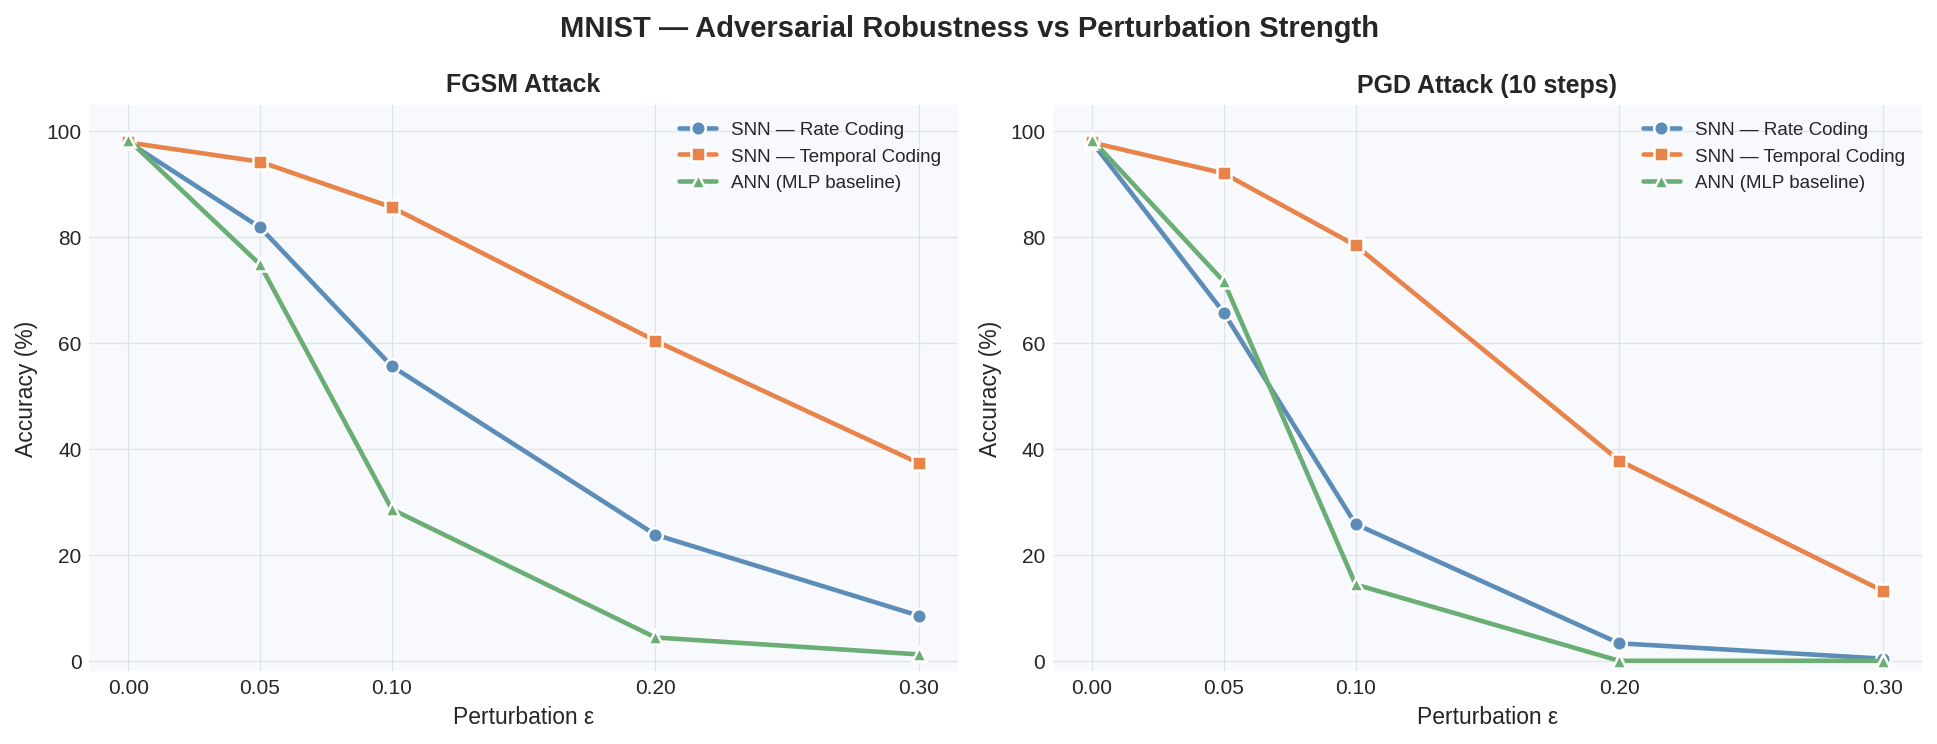
\includegraphics[width=0.9\linewidth]{fig04_mnist_robustness.png}%
    }
\end{figure}

  \begin{block}{CLEAN VS ADVERSARIAL SAMPLES}
    \begin{figure}
      \centering
      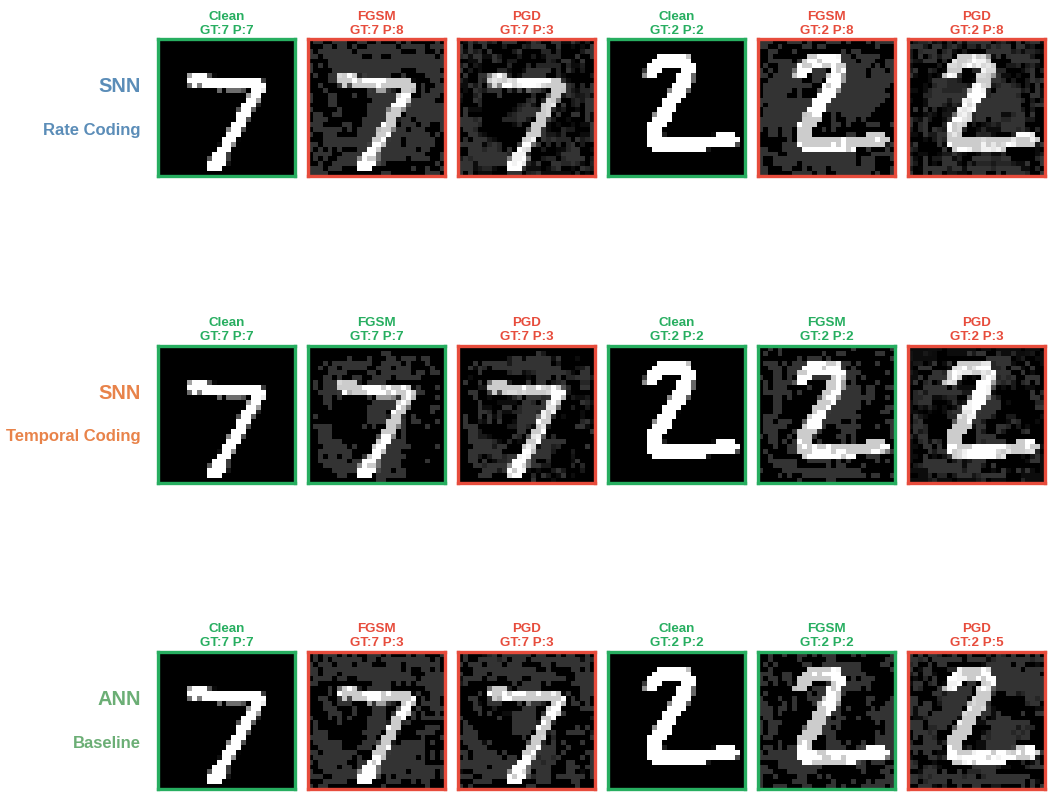
\includegraphics[width=0.9\linewidth]{fig_9_v3.png}
      \caption{\textbf{MNIST — Adversarial Samples ($\varepsilon=0.2$).}
               Rows: SNN-Rate $\cdot$ SNN-Temporal $\cdot$ ANN baseline.
               Green border = correct prediction; red = fooled.}
    \end{figure}
    \begin{figure}
      \centering
      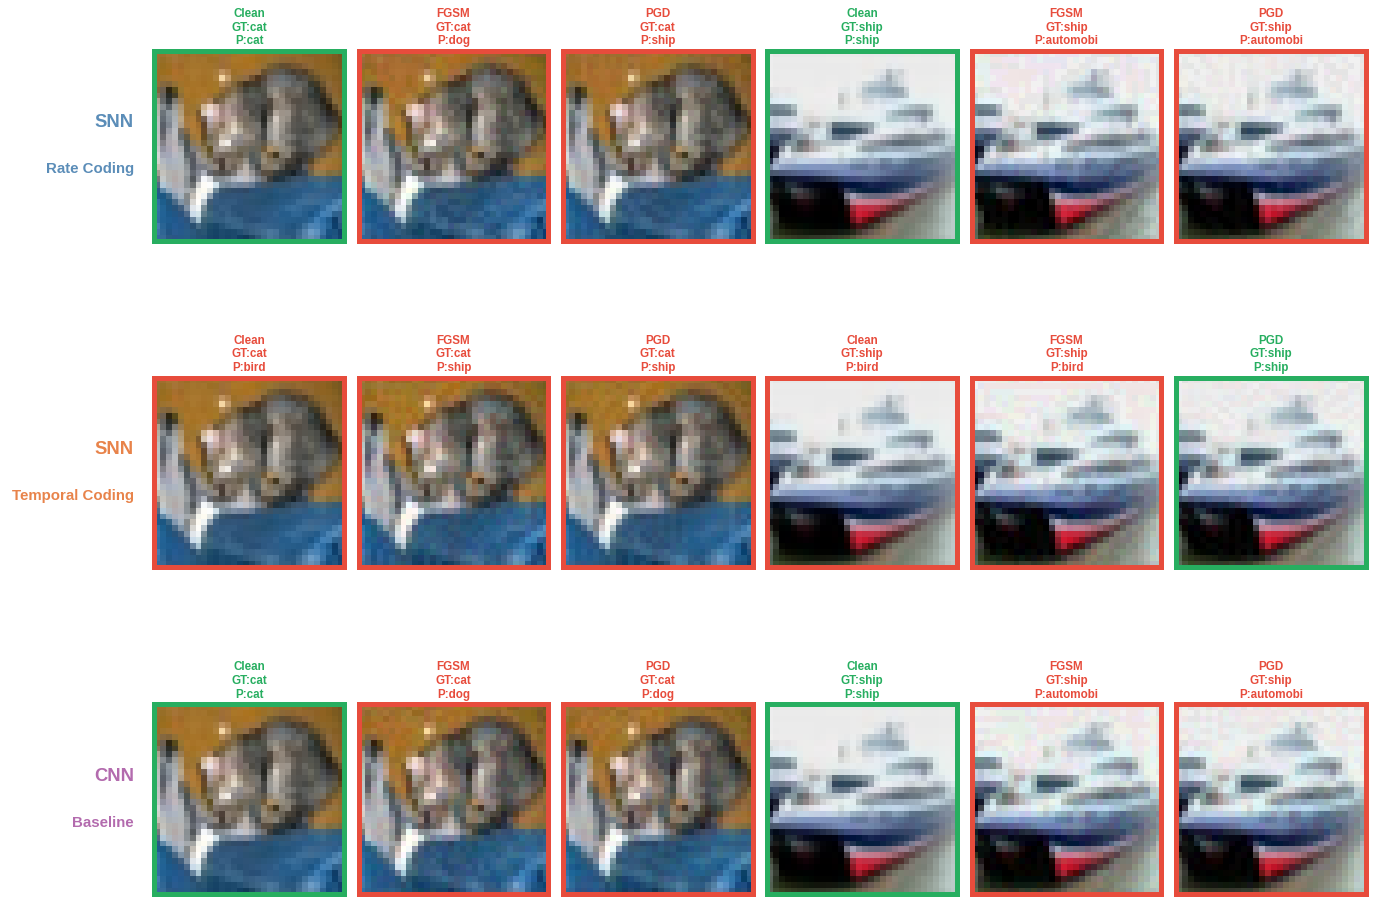
\includegraphics[width=0.9\linewidth]{fig_10_v3.png}
      \caption{\textbf{CIFAR-10 — Adversarial Samples ($\varepsilon=0.1$).}
               Rows: SNN-Rate $\cdot$ SNN-Temporal $\cdot$ CNN baseline.
               Each group: Clean $\cdot$ FGSM $\cdot$ PGD.}
    \end{figure}
  \end{block}

\end{column}

% ============================================================
% COLUMN 4: Results & Conclusion
% ============================================================
\begin{column}{\colfour}

  
    \begin{figure}
    \centering
    \fbox{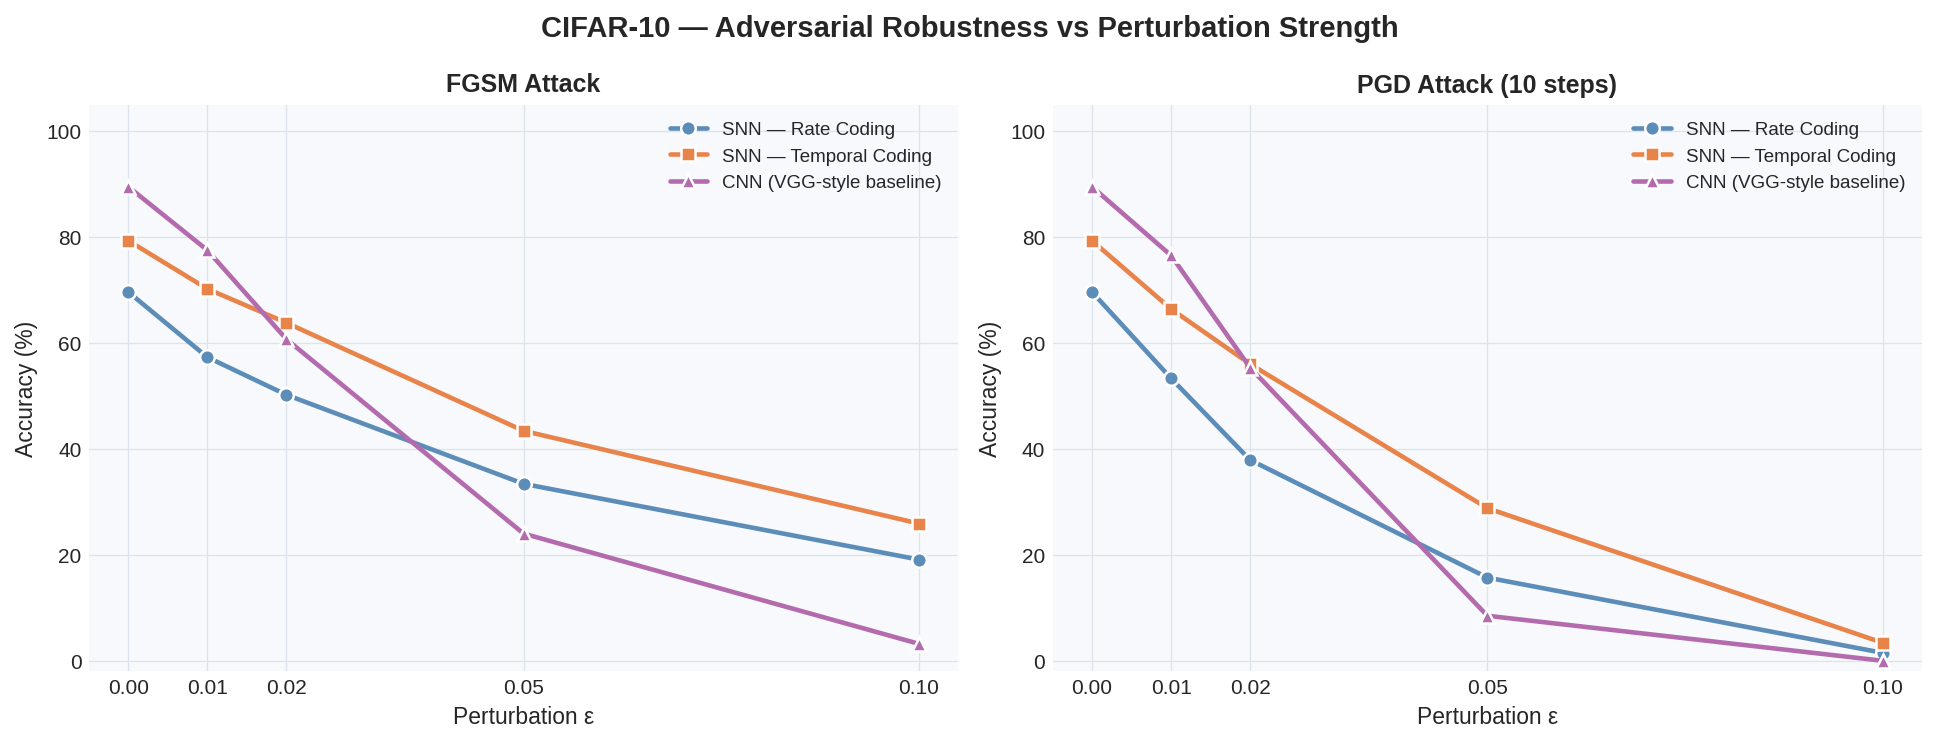
\includegraphics[width=1\linewidth]{fig05_cifar_robustness.png}}
\end{figure}
  

  \begin{block}{KEY FINDINGS}
    \begin{futurebox}
      \begin{enumerate}
        \item \textbf{Temporal $\gg$ Rate under attack.}
              MNIST: temporal retains 60.4\% (FGSM) vs.\ Rate's 23.8\%
              at $\varepsilon=0.2$ — a \textbf{+36.6 pp} advantage.
              Under PGD: 37.8\% vs.\ 3.3\% (\textbf{+34.5 pp}).

        \item \textbf{Both SNNs crush ANNs adversarially.}
              ANN collapses to 0.0\% under PGD $\varepsilon=0.2$.
              SNN-Temporal retains 37.8\%. Even SNN-Rate: 3.3\%.

        \item \textbf{PGD far stronger than FGSM.}
              SNN-Rate drops an extra \textbf{20.5 pp} from FGSM
              to PGD at $\varepsilon=0.2$. ANN already collapsed.

        \item \textbf{Temporal wins on CIFAR-10 too.}
              Despite lower clean accuracy (79.3\% vs.\ CNN's 89.5\%),
              temporal SNN retains 28.8\% under PGD vs.\ CNN's 8.5\%
              (\textbf{+20.3 pp}).

        \item \textbf{Encoding = robustness design parameter.}
              Same architecture, same training — only encoder changes,
              yet robustness gap is dramatic. Spike timing discreteness
              impedes gradient-based attacks.
      \end{enumerate}
    \end{futurebox}
  \end{block}

  \begin{block}{FUTURE WORK}
    \begin{itemize}
      \item \textbf{Adversarial training} via surrogate-gradient PGD for
            certified robust neuromorphic models.
      \item Evaluate on \textbf{larger architectures} (ResNet-SNN) and
            neuromorphic datasets (DVS-Gesture, N-MNIST).
      \item Investigate \textbf{black-box \& transfer attacks} where gradient
            sparsity advantage may differ.
      \item Explore \textbf{hybrid / population coding} robustness profiles.
      \item Robustness analysis on actual \textbf{neuromorphic hardware}
            (Intel Loihi, BrainScaleS).
    \end{itemize}
  \end{block}

  \begin{block}{REFERENCES}
    \footnotesize
    \begin{enumerate}
      \item Neftci, Mostafa \& Zenke (2019). Surrogate gradient learning in
            spiking neural networks. \textit{IEEE Signal Process.\ Mag.}
      \item Aribe (2025). Spiking Neural Networks: The Future of Brain-Inspired
            Computing. \textit{Int.\ J.\ Eng.\ Trends Technol.}
      \item Stutz (n.d.). $L_p$ adversarial examples using projected gradient
            descent in PyTorch. \textit{https://davidstutz.de/}.
    \end{enumerate}
  \end{block}
  \begin{block}{ACKNOWLEDGEMENT}
  We sincerely thank our project supervisor Prof.\ Manisha Padala for guidance and support.
      
  \end{block}

\end{column}
\end{columns}

% ---- Footer --------------------------------------------------
\begin{tikzpicture}[remember picture,overlay]
  \fill[iitgnblue]
    (current page.south west) rectangle
    ([yshift=1.85cm]current page.south east);

  \node[anchor=south, yshift=0.5cm,
        font=\small\bfseries, text=white]
    at (current page.south){%
    IIT Gandhinagar\enspace$\cdot$\enspace
    
    UG Research Showcase 2026
  };
\end{tikzpicture}

\end{frame}
\end{document}